\newcommand{\byr}{Br}

\section{Технико-экономическое обоснование эффективности разработки}

% Begin Calculations

\FPeval{\totalProgramSize}{15680}
\FPeval{\totalProgramSizeCorrected}{8650}

\FPeval{\normativeManDays}{224}

\FPeval{\additionalComplexity}{0.12}
\FPeval{\complexityFactor}{clip(1 + \additionalComplexity)}

\FPeval{\stdModuleUsageFactor}{0.7}
\FPeval{\originalityFactor}{0.7}

\FPeval{\adjustedManDaysExact}{clip( \normativeManDays * \complexityFactor * \stdModuleUsageFactor * \originalityFactor )}
\FPround{\adjustedManDays}{\adjustedManDaysExact}{0}

\FPeval{\daysInYear}{365}
\FPeval{\redLettersDaysInYear}{9}
\FPeval{\weekendDaysInYear}{104}
\FPeval{\vocationDaysInYear}{21}
\FPeval{\workingDaysInYear}{ clip( \daysInYear - \redLettersDaysInYear - \weekendDaysInYear - \vocationDaysInYear ) }

\FPeval{\developmentTimeMonths}{3}
\FPeval{\developmentTimeYearsExact}{clip(\developmentTimeMonths / 12)}
\FPround{\developmentTimeYears}{\developmentTimeYearsExact}{2}
\FPeval{\requiredNumberOfProgrammersExact}{ clip( \adjustedManDays / (\developmentTimeYears * \workingDaysInYear) + 0.5 ) }

% тут должно получаться 2 ))
\FPtrunc{\requiredNumberOfProgrammers}{\requiredNumberOfProgrammersExact}{0}

\FPeval{\tariffRateFirst}{600000}
\FPeval{\tariffFactorFst}{3.04}
\FPeval{\tariffFactorSnd}{3.48}


\FPeval{\employmentFstExact}{clip( \adjustedManDays / \requiredNumberOfProgrammers )}
\FPtrunc{\employmentFst}{\employmentFstExact}{0}

\FPeval{\employmentSnd}{clip(\adjustedManDays - \employmentFst)}


\FPeval{\workingHoursInMonth}{160}
\FPeval{\salaryPerHourFstExact}{clip( \tariffRateFirst * \tariffFactorFst / \workingHoursInMonth )}
\FPeval{\salaryPerHourSndExact}{clip( \tariffRateFirst * \tariffFactorSnd / \workingHoursInMonth )}
\FPround{\salaryPerHourFst}{\salaryPerHourFstExact}{0}
\FPround{\salaryPerHourSnd}{\salaryPerHourSndExact}{0}

\FPeval{\bonusRate}{1.5}
\FPeval{\workingHoursInDay}{8}
\FPeval{\totalSalaryExact}{clip( \workingHoursInDay * \bonusRate * ( \salaryPerHourFst * \employmentFst + \salaryPerHourSnd * \employmentSnd ) )}
\FPround{\totalSalary}{\totalSalaryExact}{0}

\FPeval{\additionalSalaryNormative}{20}

\FPeval{\additionalSalaryExact}{clip( \totalSalary * \additionalSalaryNormative / 100 )}
\FPround{\additionalSalary}{\additionalSalaryExact}{0}

\FPeval{\socialNeedsNormative}{0.5}
\FPeval{\socialProtectionNormative}{34}
\FPeval{\socialProtectionFund}{ clip(\socialNeedsNormative + \socialProtectionNormative) }

\FPeval{\socialProtectionCostExact}{clip( (\totalSalary + \additionalSalary) * \socialProtectionFund / 100 )}
\FPround{\socialProtectionCost}{\socialProtectionCostExact}{0}

\FPeval{\taxWorkProtNormative}{4}
\FPeval{\taxWorkProtCostExact}{clip( (\totalSalary + \additionalSalary) * \taxWorkProtNormative / 100 )}
\FPround{\taxWorkProtCost}{\taxWorkProtCostExact}{0}
\FPeval{\taxWorkProtCost}{0} % это считать не нужно, зануляем чтобы не менять формулы

\FPeval{\stuffNormative}{3}
\FPeval{\stuffCostExact}{clip( \totalSalary * \stuffNormative / 100 )}
\FPeval{\stuffCost}{\stuffCostExact}

\FPeval{\timeToDebugCodeNormative}{15}
\FPeval{\reducingTimeToDebugFactor}{0.3}
\FPeval{\adjustedTimeToDebugCodeNormative}{ clip( \timeToDebugCodeNormative * \reducingTimeToDebugFactor ) }

\FPeval{\oneHourMachineTimeCost}{5000}

\FPeval{\machineTimeCostExact}{ clip( \oneHourMachineTimeCost * \totalProgramSizeCorrected / 100 * \adjustedTimeToDebugCodeNormative ) }
\FPround{\machineTimeCost}{\machineTimeCostExact}{0}

\FPeval{\businessTripNormative}{15}
\FPeval{\businessTripCostExact}{ clip( \totalSalary * \businessTripNormative / 100 ) }
\FPround{\businessTripCost}{\businessTripCostExact}{0}

\FPeval{\otherCostNormative}{20}
\FPeval{\otherCostExact}{clip( \totalSalary * \otherCostNormative / 100 )}
\FPround{\otherCost}{\otherCostExact}{0}

\FPeval{\overheadCostNormative}{100}
\FPeval{\overallCostExact}{clip( \totalSalary * \overheadCostNormative / 100 )}
\FPround{\overheadCost}{\overallCostExact}{0}

\FPeval{\overallCost}{clip( \totalSalary + \additionalSalary + \socialProtectionCost + \taxWorkProtCost + \stuffCost + \machineTimeCost + \businessTripCost + \otherCost + \overheadCost ) }

\FPeval{\supportNormative}{30}
\FPeval{\softwareSupportCostExact}{clip( \overallCost * \supportNormative / 100 )}
\FPround{\softwareSupportCost}{\softwareSupportCostExact}{0}


\FPeval{\baseCost}{ clip( \overallCost + \softwareSupportCost ) }

\FPeval{\profitability}{35}
\FPeval{\incomeExact}{clip( \baseCost / 100 * \profitability )}
\FPround{\income}{\incomeExact}{0}

\FPeval{\estimatedPrice}{clip( \income + \baseCost )}

\FPeval{\localRepubTaxNormative}{3.9}
\FPeval{\localRepubTaxExact}{clip( \estimatedPrice * \localRepubTaxNormative / (100 - \localRepubTaxNormative) )}
\FPround{\localRepubTax}{\localRepubTaxExact}{0}
\FPeval{\localRepubTax}{0}

\FPeval{\ndsNormative}{20}
\FPeval{\ndsExact}{clip( (\estimatedPrice + \localRepubTax) / 100 * \ndsNormative )}
\FPround{\nds}{\ndsExact}{0}


\FPeval{\sellingPrice}{clip( \estimatedPrice + \localRepubTax + \nds )}

\FPeval{\taxForIncome}{18}
\FPeval{\incomeWithTaxes}{clip(\income * (1 - \taxForIncome / 100))}
\FPround\incomeWithTaxes{\incomeWithTaxes}{0}

% End Calculations

\subsection{Характеристика программного продукта}

Предлагаемый для внедрения программный продукт является автоматизированной мобильной информационной системой ведения карточек пациента. Данная система осуществляет учет и регистрацию различного рода заболевания пациента на территории Республики Беларусь по средствам мобильного телефона. Эта разработка оказывает огромное  влияние на область медицины, ведь это позволяет автоматизировано вести картотеку пациента, тем самым позволяя во-время реагировать на определенные отклонения здоровья пациента.

Разработка продукта осуществлена в IT-компании <<Иссофт Солюшенз>> по индивидуальному заказу. В результате внедрения предлагаемой системы удается достичь:

\begin{itemize}
  \item повышения эффективности работы медицинских сотрудников и медицинских учреждений в целом;
  \item предоставление в доступном виде информацию полной картотеки пользователю-пациенту;
  \item сокращения нецелевых расходов интеллектуальной деятельности;
  \item предоставления качественного и количественного хранения информационного обеспечения.
\end{itemize}

Разработка данного проекта связана со значительными затратами трудовых и финансовых ресурсов. В связи с этим создание и реализация данного проекта нуждается в соответствующем технико-экономическом обосновании.

Целью технико-экономического обоснования является расчет и оценка следующих показателей:

\begin{itemize}
  \item смета затрат и отпускная цена ПО;
  \item прибыль от реализации ПО;
  \item рентабельность инвестиций в разработку ПО.
\end{itemize}

В результате разработки данного программного продукта снизится трудоемкость заполнения бумажной картотеки заболеваний пациента, что и будет являться результатом от внедрения программного продукта.

\subsection{Определение объема и трудоемкости ПО}

\subsubsection{Объем ПО}

Базой для расчета плановой сметы затрат на разработку ПО является объем ПО.   

\subsubsection{Общий объем ($ V_{o} $)}

Общий объем программного продукта определяется исходя из количества и объема функций, реализуемых программой:

\begin{equation}
  \label{eq:econ:total_program_size}
  V_{o} = \sum_{i = 1}^{n} V_{i} \text{\,,}
\end{equation}
\begin{explanation}
где & $ V_{i} $ & объём отдельной функции ПО, LoC; \\
    & $ n $ & общее число функций.
\end{explanation}

\subsubsection{Единицы измерения объема ПО}

Оценивание объема программного
продукта связано с выбором наиболее подходящей единицы измерения размера продукта. В данном обосновании будет использоваться количество строк исходного кода (LinеsОfСоdе, LОС). 

Рассчитывается уточненный объем ПО ($ V_{\text{у}}$):

\begin{equation}
  \label{eq:econ:total_program_size_corrected}
  V_{\text{у}} = \sum_{i = 1}^{n} V_{i}^{\text{у}} \text{\,,}
\end{equation}
\begin{explanation}
где & $ V_{i}^{\text{y}} $ & уточненный объём отдельной функции ПО, LoC; \\
    & $ n $ & общее число функций.
\end{explanation}

Среда разработки ПО - NodeJS/Native JavaScript, ПО функционального назначения. $ V_{i}$ = 2650 LOC.


\begin{table}[ht]
\caption{Перечень и объём функций программного модуля}
\label{table:econ:function_sizes}
\centering
  \begin{tabular}{| >{\centering}m{0.12\textwidth} 
                  | >{\raggedright}m{0.40\textwidth} 
                  | >{\centering}m{0.18\textwidth} 
                  | >{\centering\arraybackslash}m{0.18\textwidth}|}

  \hline
         \multirow{2}{0.12\textwidth}[-0.5em]{\centering \No{} функции}
       & \multirow{2}{0.40\textwidth}[-0.55em]{\centering Наименование (содержание)} 
       & \multicolumn{2}{c|}{\centering Объём функции, LoC} \tabularnewline
  
  \cline{3-4} & 
       & { по каталогу ($ V_{i} $) }
       & { уточненный ($ V_{i}^{\text{у}} $) } \tabularnewline
  
  \hline 
  101 & Организация ввода информации & \num{50} & \num{50} \tabularnewline
  
  \hline
  203 & Формирование баз данных & \num{90} & \num{90} \tabularnewline

  \hline
  204 & Обработка наборов и записей баз данных & \num{300} & \num{300} \tabularnewline

  \hline
  308 & Организация крипто-сервиса & \num{900} & \num{900} \tabularnewline

  \hline
  410 & Загрузка данных & \num{550} & \num{550} \tabularnewline

  \hline
  703 & Работа с камерой моб.устройства & \num{280} & \num{280} \tabularnewline

  \hline
  705 & Формирование и вывод на внешние носители & \num{390} & \num{390} \tabularnewline

  \hline
  706 & Предварительная  обработка  и формирование PDF файлов & \num{90} & \num{90} \tabularnewline

  \hline
  Итог & & \num{2650} & \num{2650} \tabularnewline
  \hline
  \end{tabular}
\end{table}

\subsubsection{Трудоемкость разработки ПО}

По уточненному объему ПО и нормативам затрат труда в расчете на единицу объема определяются нормативная и общая трудоемкость разработки ПО.

\subsubsection{Нормативная трудоемкость разработки ПO}

На основании принятого к расчету объема (Vy) и категории сложности определяется нормативная трудоемкость ПО (Tн), которая уточняется с учетом сложности и новизны проекта и степени использования стандартных модулей при разработке.

\subsubsection{Общая трудоемкость разработки ПО}

Нормативная трудоемкость (Tн) служит основой для определения общей трудоемкости (Tо), расчет которой осуществляется различными способами в зависимости от размера проекта.

\subsubsection{Общая трудоемкость} 
Общая трудоемкость проектов рассчитывается по формуле:

\begin{equation}
  \label{eq:econ:effort_common}
  \text{Т}_\text{о} = \text{Т}_\text{н} \cdot 
                      \text{К}_\text{с} \cdot 
                      \text{К}_\text{т} \cdot 
                      \text{К}_\text{н} \text{\,,}
\end{equation}
\begin{explanation}
где & $ \text{К}_\text{с} $ & коэффициент, учитывающий сложность ПО; \\
    & $ \text{К}_\text{т} $ & поправочный коэффициент, учитывающий степень использования при разработке стандартных модулей; \\
    & $ \text{К}_\text{н} $ & коэффициент, учитывающий степень новизны ПО.
\end{explanation}

Наличие интерактивного доступа и обеспечения хранения, ведения и поиска данных в сложных структурах позволяет применить к объему ПО коэффициент Кс, который определяется по формуле:

\begin{equation}
\label{eq:econ:complexity_coeff}
  \text{К}_{\text{с}} = 1 + \sum_{i = 1}^n \text{К}_{i} \text{\,,}
\end{equation}
\begin{explanation}
где & $ \text{К}_{i} $ & коэффициент, соответствующий степени повышения сложности ПО за счет конкретной характеристики; \\
    & $ n $ & количество учитываемых характеристик.
\end{explanation}


\begin{equation}
\label{eq:econ:complexity_coeff_calc}
  \text{К}_{\text{с}} = \num{1} + \num{0,07} + \num{0,06} = \num{1,13} \text{\,.}
\end{equation}

С учетом дополнительного коэффициента сложности Кс рассчитывается общая трудоемкость ПС по формуле:
\begin{equation}
  \label{eq:econ:effort_common_calc}
  \text{Т}_\text{о} = \num{745,8} \approx \num{746}{\text{чел.}/\text{дн.}}
\end{equation}


\subsubsection{Численность исполнителей и срок разработки ПО}

На основе общей трудоемкости и требуемых сроков реализации проекта вычисляется плановое количество исполнителей. При этом могут решаться следующие задачи:

\begin{itemize}
  \item расчет числа исполнителей при заданных сроках разработки;
  \item определение сроков разработки проекта при заданной численности исполнителей.
\end{itemize}

\subsubsection{Численность исполнителей}

Численность исполнителей проекта рассчитывается по формуле:

\begin{equation}
  \label{eq:econ:num_of_programmers}
  \text{Ч}_\text{р} = \frac{\text{Т}_\text{о}}{\text{Т}_\text{р} \cdot \text{Ф}_\text{эф}} \text{\,,}
\end{equation}
\begin{explanation}
где & $ \text{Т}_\text{о} $ & общая трудоемкость разработки проекта, $ \text{чел.}/\text{дн.} $; \\
    & $ \text{Ф}_\text{эф} $ & эффективный фонд времени работы одного работника в течение года, дн.; \\
    & $ \text{Т}_\text{р} $ & срок разработки проекта, лет.
\end{explanation}

\subsubsection{Срок разработки проекта}

Срок разработки проекта рассчитывается по формуле:

\begin{equation}
  \label{eq:econ:num_of_programmers_c}
  \text{Т}_\text{р} = \frac{\text{Т}_\text{о}}{\text{Ч}_\text{р} \cdot \text{Ф}_\text{эф}} \text{\,,}
\end{equation}
\begin{explanation}
где & $ \text{Т}_\text{о} $ & общая трудоемкость разработки проекта, $ \text{чел.}/\text{дн.} $; \\
    & $ \text{Ф}_\text{эф} $ & эффективный фонд времени работы одного работника в течение года, дн.; \\
    & $ \text{Т}_\text{р} $ & срок разработки проекта, лет.
\end{explanation}


\subsubsection{Эффективный фонд времени работы}

Эффективный фонд времени работы одного работника рассчитывается по формуле:
\begin{equation}
  \label{eq:econ:effective_time_per_programmer}
  \text{Ф}_\text{эф} = 
    \text{Д}_\text{г} -
    \text{Д}_\text{п} -
    \text{Д}_\text{в} -
    \text{Д}_\text{о} \text{\,,}
\end{equation}
\begin{explanation}
где & $ \text{Д}_\text{г} $ & количество дней в году, дн.; \\
    & $ \text{Д}_\text{п} $ & количество праздничных дней в году, не совпадающих с выходными днями, дн.; \\
    & $ \text{Д}_\text{в} $ & количество выходных дней в году, дн.; \\
    & $ \text{Д}_\text{п} $ & количество дней отпуска, дн.
\end{explanation}

Трудоемкость <<Технорабочего проекта>> определяется по формуле:

\begin{equation}
  \label{eq:econ:effective_time_per_programmer_df}
  \text{Т}_\text{трп} = 
    \num{0,85} \cdot 
    \text{Т}_\text{тп} +
    \num{1} -
    \text{Т}_\text{рп} \text{\,.}
\end{equation}

Она составляет: 

\begin{equation}
  \label{eq:econ:effective_time_per_programmer_dfr}
  \text{Т}_\text{трп} = 
    \num{0,85} \cdot 
    \num{36,54} +
    \num{1} -
    \num{222,92} =
    \num{254} {\text{чел.}/\text{дн}} \text{\,.}
\end{equation}

На основе уточненной трудоемкости разработки ПС и установленного периода разработки, общая численность разработчиков равна:

\begin{equation}
  \text{Ф}_\text{эф} = \num{\daysInYear} - \num{5} - \num{106} - \num{31} = \SI{223}{\text{дня в год}}
\end{equation}

\subsection{Расчет затрат и отпускной цены программного средства}

1) Основная заработная плата исполнителей проекта определяется по формуле:
\begin{equation}
  \label{eq:econ:total_salary}
  \text{З}_{\text{о}} = \sum^{n}_{i = 1} 
                        \text{Т}_{\text{ч}}^{i} \cdot
                        \text{Т}_{\text{ч}} \cdot
                        \text{Ф}_{\text{п}} \cdot
                        \text{К}
                          \text{\,,}
\end{equation}
\begin{explanation}
где & $ \text{Т}_{\text{ч}}^{i} $ & часовая тарифная ставка \mbox{$ i $-го} исполнителя, \byr$/$час; \\
    & $ \text{Т}_{\text{ч}} $ & количество часов работы в день, час; \\
    & $ \text{Ф}_{\text{п}} $ & плановый фонд рабочего времени \mbox{$ i $-го} исполнителя, дн.; \\
    & $ \text{К} $ & коэффициент премирования.
\end{explanation}

В настоящий момент тарифная ставка 1-го разряда на предприятии составляет 700 тыс. руб. 

Расчет основной заработной платы представлен в таблице~\ref{table:econ:programmers_zp}.

\begin{table}[ht]
  \caption{Расчет основной заработной платы}
  \label{table:econ:programmers_zp}
  \begin{tabular}{| >{\raggedright}p{0.17\textwidth} 
                  | >{\raggedright}p{0.08\textwidth} 
                  | >{\raggedright}p{0.13\textwidth}
                  | >{\raggedright}p{0.12\textwidth}
                  | >{\raggedright}p{0.10\textwidth}
                  | >{\raggedright}p{0.10\textwidth} 
                  | >{\raggedright\arraybackslash}p{0.12\textwidth}|}
   \hline
   Исполнители & Разряд & Тарифный коэффициент & Месячная тарифная ставка тыс.руб. & Часовая тарифная ставка тыс.руб. & Плано-вый фонд рабочего времени, дн. & Основная заработная плата, тыс. руб.\\
   \hline
   Программист \Rmnum{2}-категории & $ \num{10} $ & $ \num{2,48} $ & $ \num{1736} $ & $ \num{28603} $& $ \num{22} $  & $ \num{5006} $\\
   
   \hline
  \end{tabular}
\end{table}

2) Дополнительная заработная плата исполнителей проекта определяется по формуле:

\begin{equation}
  \label{eq:econ:additional_salary}
  \text{З}_{\text{д}} = 
    \frac {\text{З}_{\text{о}} \cdot \text{Н}_{\text{д}}} 
          {100\%} \text{\,,}
\end{equation}
\begin{explanation}
  где & $ \text{Н}_{\text{д}} $ & норматив дополнительной заработной платы, $ \% $.
\end{explanation}

Дополнительная заработная плата составит:

\begin{equation}
  \label{eq:econ:additional_salary_calc}
  \text{З}_{\text{д}} = 
    \frac{\num{5006} \cdot 20\%}
         {100\%} \approx \SI{1 001 }{\text{тыс.руб}} \text{\,.}
\end{equation}

3) Отчисления в фонд социальной защиты населения и на обязательное страхование (ЗС) определяются в соответствии с действующими законодательными актами по формуле:

\begin{equation}
  \label{eq:econ:soc_prot}
  \text{З}_{\text{сз}} = 
    \frac{(\text{З}_{\text{о}} + \text{З}_{\text{д}}) \cdot \text{Н}_{\text{сз}}}
         {\num{100\%}} \text{\,.}
\end{equation}

Подставив вычисленные ранее значения в формулу получаем:
\begin{equation}
  \label{eq:econ:soc_prot_calc}
  \text{З}_{\text{сз}} =
    \frac{ (\num{5006} + \num{1001}) \cdot \num{34,6\%} }
         { \num{100\%} }
    \approx \SI{2078}{\text{тыс.руб}} \text{\,.}
\end{equation}

4) Расходы по статье <<Машинное время>> (РМ) включают оплату машинного времени, необходимого для разработки и отладки ПС, и определяются по формуле:

\begin{equation}
  \label{eq:econ:machine_time}
  \text{Р}_{\text{м}} =
    \text{Ц}_{\text{м}} \cdot 
    \text{Т}_{\text{ч}} \cdot 
    \text{С}_{\text{р}}
    \text{\,,}
\end{equation}
\begin{explanation}
  где & $ \text{Ц}_{\text{м}} $ & цена одного часа машинно-часа, бел.руб.; \\
      & $ \text{Т}_{\text{ч}} $ & количество часов работы в день; \\
      & $ \text{С}_{\text{р}} $ & длительность проекта.
\end{explanation}

Стоимость машино-часа на предприятии составляет 6 тыс. руб.. Разработка проекта займет 90 дней. Определим затраты по статье <<Машинное время>>:

\begin{equation}
  \label{eq:econ:machine_time}
  \text{Р}_{\text{м}} =
    \num{6} \cdot 
    \num{4} \cdot 
    \num{88} =
    \SI{2112}{\text{тыс.руб}} \text{\,.}
\end{equation}


5) Затраты по статье <<Накладные расходы>> (РН), определяются по формуле:

\begin{equation}
  \label{eq:econ:overhead_cost}
  \text{Р}_{\text{н}} =
    \frac{ \text{З}_{\text{о}} \cdot \text{Н}_{\text{рн}} }
         { \num{100\%} } \text{\,,}
\end{equation}
\begin{explanation}
  где & $ \text{Н}_{\text{рн}} $ & норматив накладных расходов в организации,~$ \num{50\%} $.
\end{explanation}

Накладные расходы составят:

\begin{equation}
  \label{eq:econ:overhead_cost_calc}
  \text{Р}_{\text{н}} =
   \text{Р}_{\text{н}} =
    \num{5006} \cdot 
    \num{0.5} = 
    \SI{2503}{\text{тыс.руб}} \text{\,.}
\end{equation}

Общая сумма расходов по всем статьям сметы (Сп) на ПО рассчитывается по формуле:

\begin{equation}
  \label{eq:econ:overall_cost}
  \text{С}_{\text{р}} =
    \text{З}_{\text{о}} +
    \text{З}_{\text{д}} +
    \text{З}_{\text{сз}} +
    \text{Р}_{\text{м}} +
    \text{Р}_{\text{н}}\text{\,.}
\end{equation}

Подставляя ранее вычисленные значения в формулу получаем:
\begin{equation}
  \label{eq:econ:overall_cost_calc}
  \text{С}_{\text{р}} =
    \num{5006} \cdot 
    \num{1001} \cdot 
    \num{2078} \cdot 
    \num{2112} \cdot 
    \num{2503} = \SI{12699,8}{\text{тыс. руб}} \text{\,.}
\end{equation}

Расходы на сопровождение и адаптацию, которые несет производитель ПО, вычисляются по нормативу от суммы расходов по смете и рассчитываются по формуле:
\begin{equation}
  \label{eq:econ:software_support}
  \text{Р}_{\text{са}} = 
    \frac { \text{С}_{\text{р}} \cdot \text{Н}_{\text{рса}} }
          { \num{100\%} } \text{\,,}
\end{equation}
\begin{explanation}
  где & $ \text{Н}_{\text{рса}} $ & норматив расходов на сопровождение и адаптацию ПО,~$ \num{20\%} $.
\end{explanation}


\begin{equation}
  \label{eq:econ:software_support_calc}
  \text{Р}_{\text{са}} = 
    \frac { \num{12699,8} \cdot \num{20\%} }
          { \num{100\%} } \approx \SI{2540}{\text{тыс. руб}} \text{\,.}
\end{equation}

Общая сумма расходов на разработку (с затратами на сопровождение и адаптацию) как полная себестоимость ПС (СП) определяется по формуле:

\begin{equation}
  \label{eq:econ:base_cost}
  \text{С}_{\text{п}} = \text{С}_{\text{р}} + \text{Р}_{\text{са}} \text{\,.}
\end{equation}

Подставляя известные значения в формулу получаем:
\begin{equation}
  \label{eq:econ:base_cost_calc}
  \text{С}_{\text{п}} = \num{12700} + \num{2540} = \SI{15240}{\text{тыс. руб}} \text{\,.}
\end{equation}

Прибыль ПС рассчитывается по формуле:

\begin{equation}
  \label{eq:econ:income}
  \text{П}_{\text{с}} = 
    \frac { \text{С}_{\text{п}} \cdot \text{У}_{\text{р}} }
          { \num{100\%} } \text{\,,}
\end{equation}
\begin{explanation}
  где & $ \text{П}_{\text{с}} $ & прибыль от реализации ПО заказчику, тыс.руб.; \\
      & $ \text{У}_{\text{р}} $ & уровень рентабельности ПО,~$ \num{25\%} $; \\
      & $ \text{С}_{\text{п}} $ & себестоимость ПС (руб.).
\end{explanation}

Подставив известные данные в формулу получаем:
\begin{equation}
  \label{eq:econ:income_calc}
  \text{П}_{\text{с}} = 
    \frac { \num{15240} \cdot \num{25\%} }
          { \num{100\%} } 
    \approx \SI{3810}{\text{тыс.руб}} \text{\,.}
\end{equation}

Прогнозируемая отпускная цена ПС:
\begin{equation}
  \label{eq:econ:estimated_price}
  \text{Ц}_{\text{п}} = \text{С}_{\text{п}} + \text{П}_{\text{с}}  \text{\,.}
\end{equation}

Подставив данные в формулу получаем:
\begin{equation}
  \label{eq:econ:estimated_price_calc}
  \text{Ц}_{\text{п}} = \num{15240}  + \num{3810} = \SI{19050}{\text{тыс.руб}} \text{\,.}
\end{equation}

\subsection{Расчет стоимостной оценки результата}

Результатом (Р) в сфере использования программного продукта является прирост чистой прибыли и амортизационных отчислений.

\subsubsection{Расчет прироста чистой прибыли}

1) Экономия затрат на заработную плату при использовании ПС в расчете на объем выполняемых работ определяется по формуле:

\begin{equation}
  \label{eq:econ:incomex}
  \text{Э}_{\text{з}} = 
    \text{К}_{\text{пр}} \cdot 
    (\text{Т}_{\text{с}} \cdot  \text{ТС} - \text{Т}_{\text{н}} \cdot  \text{ТН}) \cdot 
    \text{N}_{\text{п}} \cdot 
    (\num{1} + \text{Н}_{\text{д}}/\num{100}) \cdot 
    (\num{1} + \text{Н}_{\text{но}}/\num{100})\text{\,,}
\end{equation}
\begin{explanation}
  где & $ \text{Т}_{\text{с}} $, $ \text{Т}_{\text{н}} $ & трудоемкость выполнения работы до и после внедрения программного продукта, нормо-час; \\
      & $ \text{ТС} $, $ \text{ТН} $ & часовая тарифная ставка, соответствующая разряду выполняемых работ до и после внедрения программного продукта, тыс. руб./ч.; \\
      & $ \text{К}_{\text{пр}} $ & коэффициент премий; \\
      & $ \text{Н}_{\text{д}} $ & норматив дополнительной заработной платы; \\
      & $ \text{Н}_{\text{но}} $ & ставка отчислений от заработной платы, включаемых в себестоимость. \\
\end{explanation}

До внедрения программного продукта трудоемкость регистрации недвижимого имущества составляла 1,3 человека-часа, после внедрения программы – 0,5 человека-часа. В год предприятие проводит около 1500 регистраций недвижимого имущества.  
Экономия на заработной и начисления на заработную плату составит:

\begin{equation}
  \label{eq:econ:estimated_price_calcdd}
  \text{Э}_{\text{з}} = \num{1,35} \cdot  (\num{1,3} \cdot  \num{8002} - \num{0,5} \cdot  \num{8002}) \cdot  \num{300} \cdot  \num{1,2} \cdot  \num{1,346} = \SI{4188}{\text{тыс.руб}} \text{\,.}
\end{equation}

Прирост чистой прибыли (ΔПч) определяется по формуле:

\begin{equation}
  \label{eq:econ:incomex}
  \text{ΔП}_{\text{ч}} = 
    \text{С}_{\text{о}} -
    ((\text{С}_{\text{о}} \cdot  \text{Н}_{\text{п}})/100)\text{\,,}
\end{equation}
\begin{explanation}
  где & $ \text{Н}_{\text{п}} $ & ставка налога на прибыль; \\
\end{explanation}

Таким образом, прирост чистой прибыли составит:

\begin{equation}
  \label{eq:econ:estimated_price_calcdd}
  \text{ΔП}_{\text{ч}} = \num{4990} - \num{4188} \cdot  \num{18} / \num{100} = \SI{4237}{\text{тыс.руб}} \text{\,,}
\end{equation}
  
\subsubsection{Расчет прироста амортизационных отчислений}

Расчет амортизационных отчислений осуществляется по формуле:

\begin{equation}
  \label{eq:econ:incomex}
  \text{А} = 
    \text{Н}_{\text{а}} \cdot 
    ((\text{З}/100)\text{\,.}
\end{equation}
\begin{explanation}
  где & $ \text{З} $ & затраты на разработку программы, тыс. руб.; \\
      & $ \text{Н}_{\text{а}} $ & норма амортизации программного продукта. \\
\end{explanation}

Таким образом, получим:

\begin{equation}
  \label{eq:econ:estimated_price_calcdd}
  \text{А} = \num{19050} \cdot  \num{0,2} = \SI{3810}{\text{тыс.руб}} \text{\,}
\end{equation}

\subsection{Расчет показателей эффективности использования программного продукта}

Для расчета показателей экономической эффективности использования программного продукта необходимо полученные суммы результата (прироста чистой прибыли) и затрат (капитальных вложений) по годам приводят к единому времени – расчетному году (за расчетный год принят 2015 год) путем умножения результатов и затрат за каждый год на коэффициент привидения ($ \text{ALFA}_{\text{t}} $), который рассчитывается по формуле:


\begin{equation}
  \label{eq:econ:incomex}
  \text{ALFA}_{\text{t}} = 
    (\num{1} + \text{E}_{\text{н}})^{\text{t}_{\text{p}} - \text{t}}\text{\,,}
\end{equation}
\begin{explanation}
  где & $ \text{E}_{\text{н}} $ & норматив привидения разновременных затрат и результатов; \\
      & $ \text{t}_{\text{p}} $ & расчетный год. \\
\end{explanation}

Результаты расчета показателей эффективности приведены в таблице 7.3.

Проект планируется внедрить в организации во второй половине 2016 года, поэтому в 2016 году организация может получить половину прибыли.

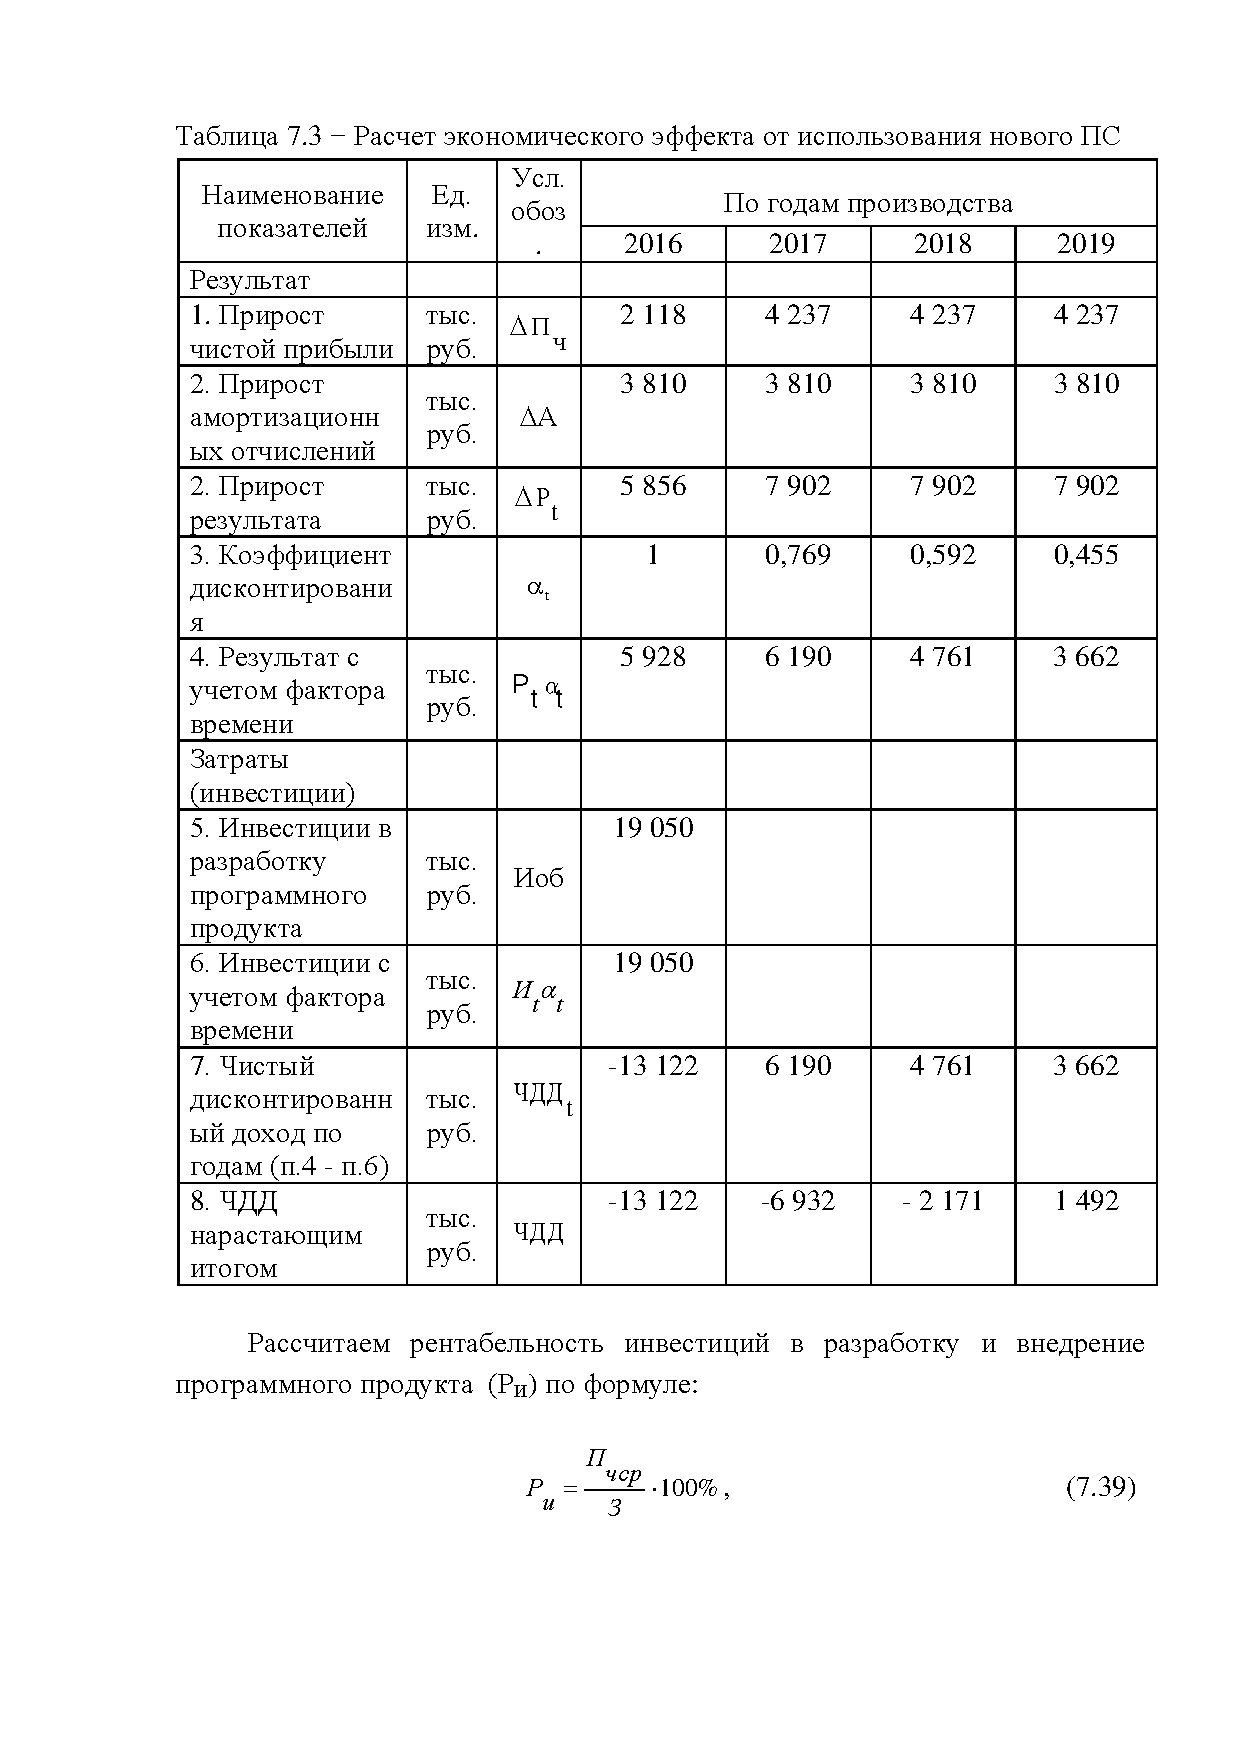
\includepdf[pages={-}, pagecommand={}]{economic_table.pdf}

\FPeval{\firstYearVariableCosts}{17200}
\FPeval{\secondYearVariableCosts}{18300}
\FPeval{\thirdYearVariableCosts}{15800}

\FPeval{\firstYearConstCosts}{12000}
\FPeval{\secondYearConstCosts}{11100}
\FPeval{\thirdYearConstCosts}{9400}

\FPeval{\firstYearCostOfProduction}{clip(\firstYearVariableCosts + \firstYearConstCosts)}
\FPeval{\secondYearCostOfProduction}{clip(\secondYearVariableCosts + \secondYearConstCosts)}
\FPeval{\thirdYearCostOfProduction}{clip(\thirdYearVariableCosts + \thirdYearConstCosts)}

\FPeval{\firstYearGrossProfit}{clip(\revenueInFirstYear - \firstYearCostOfProduction)}
\FPeval{\secondYearGrossProfit}{clip(\revenueInSecondYear - \secondYearCostOfProduction)}
\FPeval{\thirdYearGrossProfit}{clip(\revenueInThirdYear - \thirdYearCostOfProduction)}

\FPeval{\firstYearPropertyTax}{300}
\FPeval{\secondYearPropertyTax}{300}
\FPeval{\thirdYearPropertyTax}{300}

\FPeval{\firstYearTaxableIncome}{clip(\firstYearGrossProfit - \firstYearPropertyTax)}
\FPeval{\secondYearTaxableIncome}{clip(\secondYearGrossProfit - \secondYearPropertyTax)}
\FPeval{\thirdYearTaxableIncome}{clip(\thirdYearGrossProfit - \thirdYearPropertyTax)}

\FPeval{\incomeTax}{0.12}
\FPeval{\fyIncomeTax}{clip(\firstYearTaxableIncome * \incomeTax)}
\FPeval{\syIncomeTax}{clip(\secondYearTaxableIncome * \incomeTax)}
\FPeval{\tyIncomeTax}{clip(\thirdYearTaxableIncome * \incomeTax)}

\FPeval{\fyNetIncome}{clip(\firstYearTaxableIncome - \fyIncomeTax)}
\FPeval{\syNetIncome}{clip(\secondYearTaxableIncome - \syIncomeTax)}
\FPeval{\tyNetIncome}{clip(\thirdYearTaxableIncome - \tyIncomeTax)}

\FPeval{\capitalInvestments}{clip(\baseCost / 1000)}
\FPround\capitalInvestments{\capitalInvestments}{0}

\FPeval{\discountRate}{0.295}

\FPeval{\zyDiscountFactor}{1}
\FPeval{\fyDiscountFactor}{clip(\zyDiscountFactor / (1 + \discountRate))}
\FPeval{\syDiscountFactor}{clip(\fyDiscountFactor / (1 + \discountRate))}
\FPeval{\tyDiscountFactor}{clip(\syDiscountFactor / (1 + \discountRate))}


\FPeval{\fyCashFlowOutcome}{clip(\firstYearCostOfProduction + \firstYearPropertyTax + \fyIncomeTax)}
\FPeval{\syCashFlowOutcome}{clip(\secondYearCostOfProduction + \secondYearPropertyTax + \syIncomeTax)}
\FPeval{\tyCashFlowOutcome}{clip(\thirdYearCostOfProduction + \thirdYearPropertyTax + \tyIncomeTax)}

\FPeval{\fyCashFlowOutcomeDiscounted}{clip(\fyCashFlowOutcome * \fyDiscountFactor)}
\FPeval{\syCashFlowOutcomeDiscounted}{clip(\syCashFlowOutcome * \syDiscountFactor)}
\FPeval{\tyCashFlowOutcomeDiscounted}{clip(\tyCashFlowOutcome * \tyDiscountFactor)}

\FPeval{\fyCashFlowIncomeDiscounted}{clip(\firstYearCashFlowIncome * \fyDiscountFactor)}
\FPeval{\syCashFlowIncomeDiscounted}{clip(\secondYearCashFlowIncome * \syDiscountFactor)}
\FPeval{\tyCashFlowIncomeDiscounted}{clip(\thirdYearCashFlowIncome * \tyDiscountFactor)}

\FPround\fyDiscountFactor{\fyDiscountFactor}{3}
\FPround\syDiscountFactor{\syDiscountFactor}{3}
\FPround\tyDiscountFactor{\tyDiscountFactor}{3}

\FPround\fyCashFlowIncomeDiscounted{\fyCashFlowIncomeDiscounted}{0}
\FPround\syCashFlowIncomeDiscounted{\syCashFlowIncomeDiscounted}{0}
\FPround\tyCashFlowIncomeDiscounted{\tyCashFlowIncomeDiscounted}{0}

\FPround\fyCashFlowOutcomeDiscounted{\fyCashFlowOutcomeDiscounted}{0}
\FPround\syCashFlowOutcomeDiscounted{\syCashFlowOutcomeDiscounted}{0}
\FPround\tyCashFlowOutcomeDiscounted{\tyCashFlowOutcomeDiscounted}{0}

\FPround\zyNetIncomeAcc{-\capitalInvestments}{0}
\FPeval{\fyNetIncomeAcc}{clip(\zyNetIncomeAcc + (\fyCashFlowIncomeDiscounted - \fyCashFlowOutcomeDiscounted))}
\FPeval{\syNetIncomeAcc}{clip(\fyNetIncomeAcc + (\syCashFlowIncomeDiscounted - \syCashFlowOutcomeDiscounted))}
\FPeval{\tyNetIncomeAcc}{clip(\syNetIncomeAcc + (\tyCashFlowIncomeDiscounted - \tyCashFlowOutcomeDiscounted))}

